% meta.concepts: dry friction
% meta.tags: realistic
% acknowledge: Peter Seiler & Luke Melander graciously shared Spring 2019 course material
% source: 2019 P. Seiler AEM2011 HW 11

\noindent Imagine that you are a material scientist working for a popular car tire manufacturer. You will design material-level properties, in particular the coefficients of static and kinetic friction between the rubber and the road, given higher-level requirements on the car. 

\noindent The car, shown in the figure below, has a mass of 1,000kg. The center of gravity of the car is located 0.5m from the road, 1m from the forward axle, and 1.5m from the rear axle. In answering the following questions, you may assume that the car is two-dimensional (i.e. you do not have to split the forces on the tires to account for the set of left/right or driver/passenger tires).

\begin{enumerate}
  \item The car company is concerned about the maximum steepness of the slopes on which its cars can be parked. Choose the coefficient of static friction such that the cars can be parked on ramps ranging in inclination from $0^\circ$ to $40^\circ$.  
  \item Given that the car is parked on a ramp of inclination $35^\circ$, find the normal reactions and friction forces on both the front and rear tires.
\end{enumerate}

\begin{figure}[ht!]
  \centering
  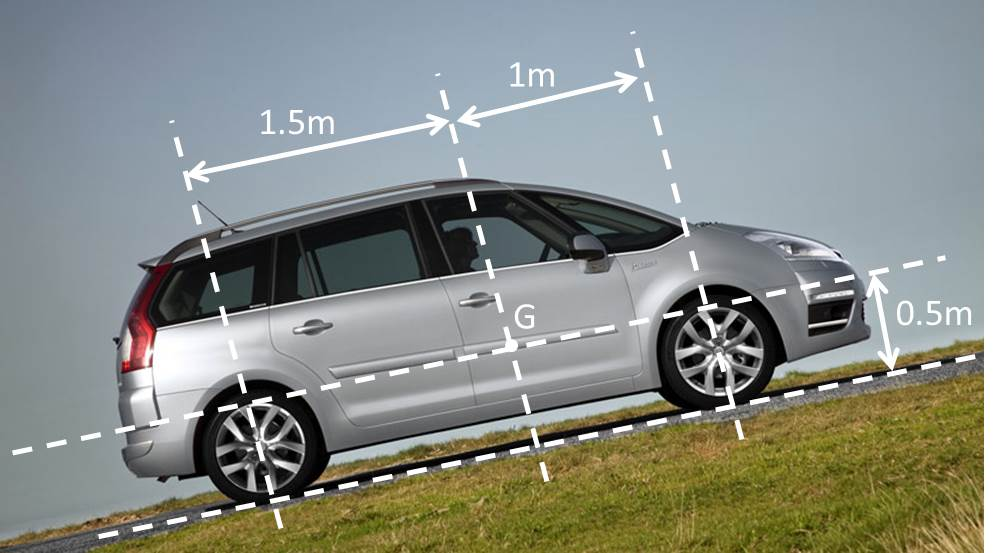
\includegraphics[width=0.5\textwidth,
	           height=0.2\textheight,
		   keepaspectratio]{fig.png}
\end{figure}


